%% ----------------------------------------------------------------
%% Thesis.tex -- MAIN FILE (the one that you compile with LaTeX)
%% ---------------------------------------------------------------- 

% Set up the document
\documentclass[a4paper, 11pt, oneside]{Thesis}  % Use the "Thesis" style, based on the ECS Thesis style by Steve Gunn
\graphicspath{{./Figures/}}  % Location of the graphics files (set up for graphics to be in PDF format)
\usepackage{float}
% Include any extra LaTeX packages required
\usepackage[style=authoryear,backend=biber]{biblatex} 
\addbibresource{Bibliography.bib}  % The references (bibliography) information are stored in the file named "Bibliography.bib"
\usepackage{amsmath}% mathtools includes this so this is optional

% Please add the following required packages to your document preamble:
 \usepackage{booktabs}
 \usepackage{multirow}
 \usepackage{pdflscape}
\usepackage{afterpage}
\usepackage{csquotes}

\usepackage{multicol}

\usepackage{verbatim}  % Needed for the "comment" environment to make LaTeX comments
\usepackage{vector}  % Allows "\bvec{}" and "\buvec{}" for "blackboard" style bold vectors in maths
\hypersetup{urlcolor=blue, colorlinks=true}  % Colours hyperlinks in blue, but this can be distracting if there are many links.

%% ----------------------------------------------------------------
\begin{document}
\frontmatter      % Begin Roman style (i, ii, iii, iv...) page numbering

% Set up the Title Page
\title  {Development of a Destination Choice Model for Ontario}
\authors  {Joseph Molloy}
\addresses  {\groupname\\\deptname\\\univname}  % Do not change this here, instead these must be set in the "Thesis.cls" file, please look through it instead
\date       {\today}
\subject    {}
\keywords   {}

\maketitle
%% ----------------------------------------------------------------

\setstretch{1.3}  % It is better to have smaller font and larger line spacing than the other way round

% Define the page headers using the FancyHdr package and set up for one-sided printing
\fancyhead{}  % Clears all page headers and footers
\rhead{\thepage}  % Sets the right side header to show the page number
\lhead{}  % Clears the left side page header

\pagestyle{fancy}  % Finally, use the "fancy" page style to implement the FancyHdr headers

%% ----------------------------------------------------------------
% Declaration Page required for the Thesis, your institution may give you a different text to place here
\Declaration{

\addtocontents{toc}{\vspace{1em}}  % Add a gap in the Contents, for aesthetics

I, AUTHOR NAME, declare that this thesis titled, `THESIS TITLE' and the work presented in it are my own. I confirm that:

\begin{itemize} 
\item[\tiny{$\blacksquare$}] This work was done wholly or mainly while in candidature for a research degree at this University.
 
\item[\tiny{$\blacksquare$}] Where any part of this thesis has previously been submitted for a degree or any other qualification at this University or any other institution, this has been clearly stated.
 
\item[\tiny{$\blacksquare$}] Where I have consulted the published work of others, this is always clearly attributed.
 
\item[\tiny{$\blacksquare$}] Where I have quoted from the work of others, the source is always given. With the exception of such quotations, this thesis is entirely my own work.
 
\item[\tiny{$\blacksquare$}] I have acknowledged all main sources of help.
 
\item[\tiny{$\blacksquare$}] Where the thesis is based on work done by myself jointly with others, I have made clear exactly what was done by others and what I have contributed myself.
\\
\end{itemize}
 
 
Signed:\\
\rule[1em]{25em}{0.5pt}  % This prints a line for the signature
 
Date:\\
\rule[1em]{25em}{0.5pt}  % This prints a line to write the date
}
\clearpage  % Declaration ended, now start a new page

%% ----------------------------------------------------------------
% The "Funny Quote Page"
\pagestyle{empty}  % No headers or footers for the following pages

\null\vfill
% Now comes the "Funny Quote", written in italics
\textit{``Write a funny quote here.''}

\begin{flushright}
If the quote is taken from someone, their name goes here
\end{flushright}

\vfill\vfill\vfill\vfill\vfill\vfill\null
\clearpage  % Funny Quote page ended, start a new page
%% ----------------------------------------------------------------

% The Abstract Page
\addtotoc{Abstract}  % Add the "Abstract" page entry to the Contents
\abstract{
\addtocontents{toc}{\vspace{1em}}  % Add a gap in the Contents, for aesthetics

The Thesis Abstract is written here (and usually kept to just this page). The page is kept centered vertically so can expand into the blank space above the title too\ldots

}

\clearpage  % Abstract ended, start a new page
%% ----------------------------------------------------------------

\setstretch{1.3}  % Reset the line-spacing to 1.3 for body text (if it has changed)

% The Acknowledgements page, for thanking everyone
\acknowledgements{
\addtocontents{toc}{\vspace{1em}}  % Add a gap in the Contents, for aesthetics

The acknowledgements and the people to thank go here, don't forget to include your project advisor\ldots

}
\clearpage  % End of the Acknowledgements
%% ----------------------------------------------------------------

\pagestyle{fancy}  %The page style headers have been "empty" all this time, now use the "fancy" headers as defined before to bring them back


%% ----------------------------------------------------------------
\lhead{\emph{Contents}}  % Set the left side page header to "Contents"
\tableofcontents  % Write out the Table of Contents

%% ----------------------------------------------------------------
\lhead{\emph{List of Figures}}  % Set the left side page header to "List if Figures"
\listoffigures  % Write out the List of Figures

%% ----------------------------------------------------------------
\lhead{\emph{List of Tables}}  % Set the left side page header to "List of Tables"
\listoftables  % Write out the List of Tables

%% ----------------------------------------------------------------
\setstretch{1.5}  % Set the line spacing to 1.5, this makes the following tables easier to read
\clearpage  % Start a new page
\lhead{\emph{Abbreviations}}  % Set the left side page header to "Abbreviations"
\listofsymbols{ll}  % Include a list of Abbreviations (a table of two columns)
{
% \textbf{Acronym} & \textbf{W}hat (it) \textbf{S}tands \textbf{F}or \\
\textbf{LAH} & \textbf{L}ist \textbf{A}bbreviations \textbf{H}ere \\

}

%% ----------------------------------------------------------------
% End of the pre-able, contents and lists of things
% Begin the Dedication page

\setstretch{1.3}  % Return the line spacing back to 1.3

\pagestyle{empty}  % Page style needs to be empty for this page

\addtocontents{toc}{\vspace{2em}}  % Add a gap in the Contents, for aesthetics


%% ----------------------------------------------------------------
\mainmatter	  % Begin normal, numeric (1,2,3...) page numbering
\pagestyle{fancy}  % Return the page headers back to the "fancy" style

% Include the chapters of the thesis, as separate files
% Just uncomment the lines as you write the chapters
\fancyhead[L]{\rightmark}

\input{Chapters/Litreview} % Introduction

\input{Chapters/Data} % Introduction


\input{Chapters/Estimation}

\input{Chapters/Implementation}

\input{Chapters/Epilogue}
%% ----------------------------------------------------------------
% Now begin the Appendices, including them as separate files

\addtocontents{toc}{\vspace{2em}} % Add a gap in the Contents, for aesthetics

\appendix % Cue to tell LaTeX that the following 'chapters' are Appendices

\chapter{Further data analysis}

%TODO include maps of zones, and tables of population and empoyment values etc
%TODO sections and horizonal lines in appendicies
\begin{figure}[H]
\centering
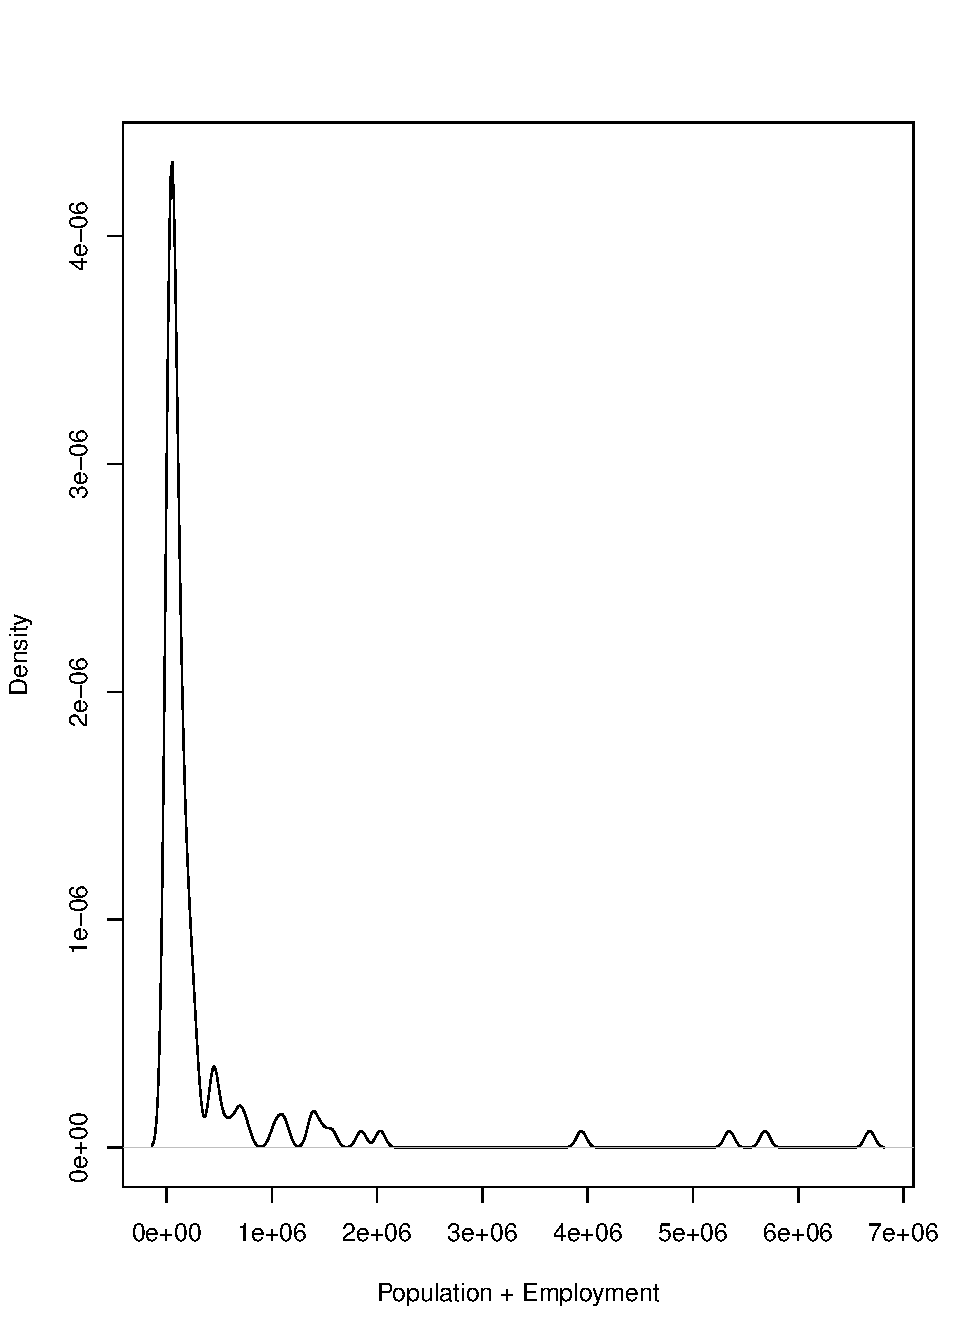
\includegraphics[height=0.6\textheight]{popEmpDensity}
\caption{Long tail and right skew of (population + employment) for each destination}
\label{fig:pop-emp-density}
\end{figure}


\begin{figure}[H]
\centering
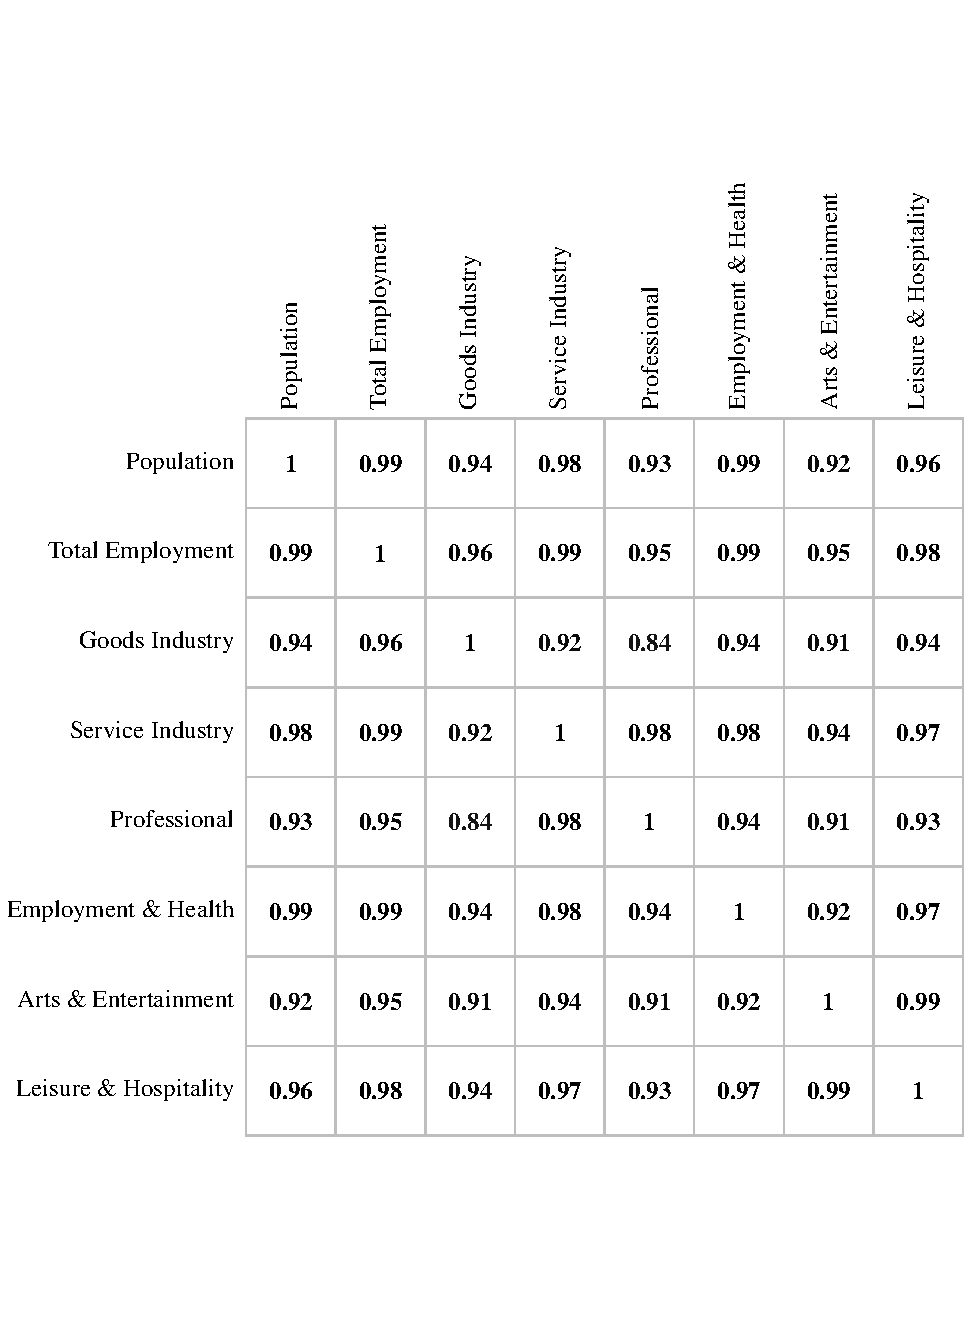
\includegraphics[width=\textwidth]{employment_correlation_plot}
\caption{High correlation between population, employment, and various employment categories across destinations}
\label{fig:pop-emp-correlation}
\end{figure}

\begin{table}[ht]
\caption{\textit{m2} Results. \\Toronto: zones 20-22, Niagara: zone 30}
\label{table:m2-error-table}
\centering
\begin{tabular}{rrrlrrrr}
  \toprule
 & Origin & Destination & Type & Predicted & Observed & Absolute Error & Max Rel. Error \\ 
  \midrule
1 & 21 & 30 & II & 877.21 & 3695.07 & 2817.86 & 3.21 \\ 
  2 & 85 & 72 & EE & 123.67 & 2407.73 & 2284.06 & 18.47 \\ 
  3 & 21 & 20 & II & 4507.84 & 2251.48 & 2256.36 & 1.00 \\ 
  4 & 21 & 22 & II & 4844.63 & 2680.21 & 2164.42 & 0.81 \\ 
  5 & 36 & 21 & II & 1346.76 & 3085.23 & 1738.46 & 1.29 \\ 
  6 & 103 & 4 & EI & 541.86 & 2061.78 & 1519.92 & 2.80 \\ 
  7 & 103 & 21 & EI & 198.15 & 1529.83 & 1331.68 & 6.72 \\ 
  8 & 21 & 53 & II & 821.51 & 2115.53 & 1294.01 & 1.58 \\ 
  9 & 64 & 64 & II & 209.47 & 1423.02 & 1213.55 & 5.79 \\ 
  10 & 21 & 54 & II & 215.05 & 1346.02 & 1130.97 & 5.26 \\ 
  11 & 20 & 30 & II & 261.47 & 1365.27 & 1103.80 & 4.22 \\ 
  12 & 22 & 30 & II & 352.63 & 1420.03 & 1067.40 & 3.03 \\ 
  13 & 30 & 30 & II & 157.40 & 1178.94 & 1021.54 & 6.49 \\ 
  14 & 21 & 52 & II & 804.06 & 1818.06 & 1014.00 & 1.26 \\ 
  15 & 21 & 4 & II & 264.90 & 1238.33 & 973.43 & 3.67 \\ 
  16 & 29 & 21 & II & 1165.79 & 2124.10 & 958.31 & 0.82 \\ 
  17 & 29 & 30 & II & 428.45 & 1353.10 & 924.65 & 2.16 \\ 
  18 & 4 & 21 & II & 403.14 & 1318.43 & 915.28 & 2.27 \\ 
  19 & 47 & 21 & II & 631.84 & 1535.96 & 904.12 & 1.43 \\ 
  20 & 4 & 85 & IE & 1660.31 & 809.08 & 851.23 & 1.05 \\ 
   \bottomrule
\end{tabular}
\end{table}

\begin{figure}[H]
\centering
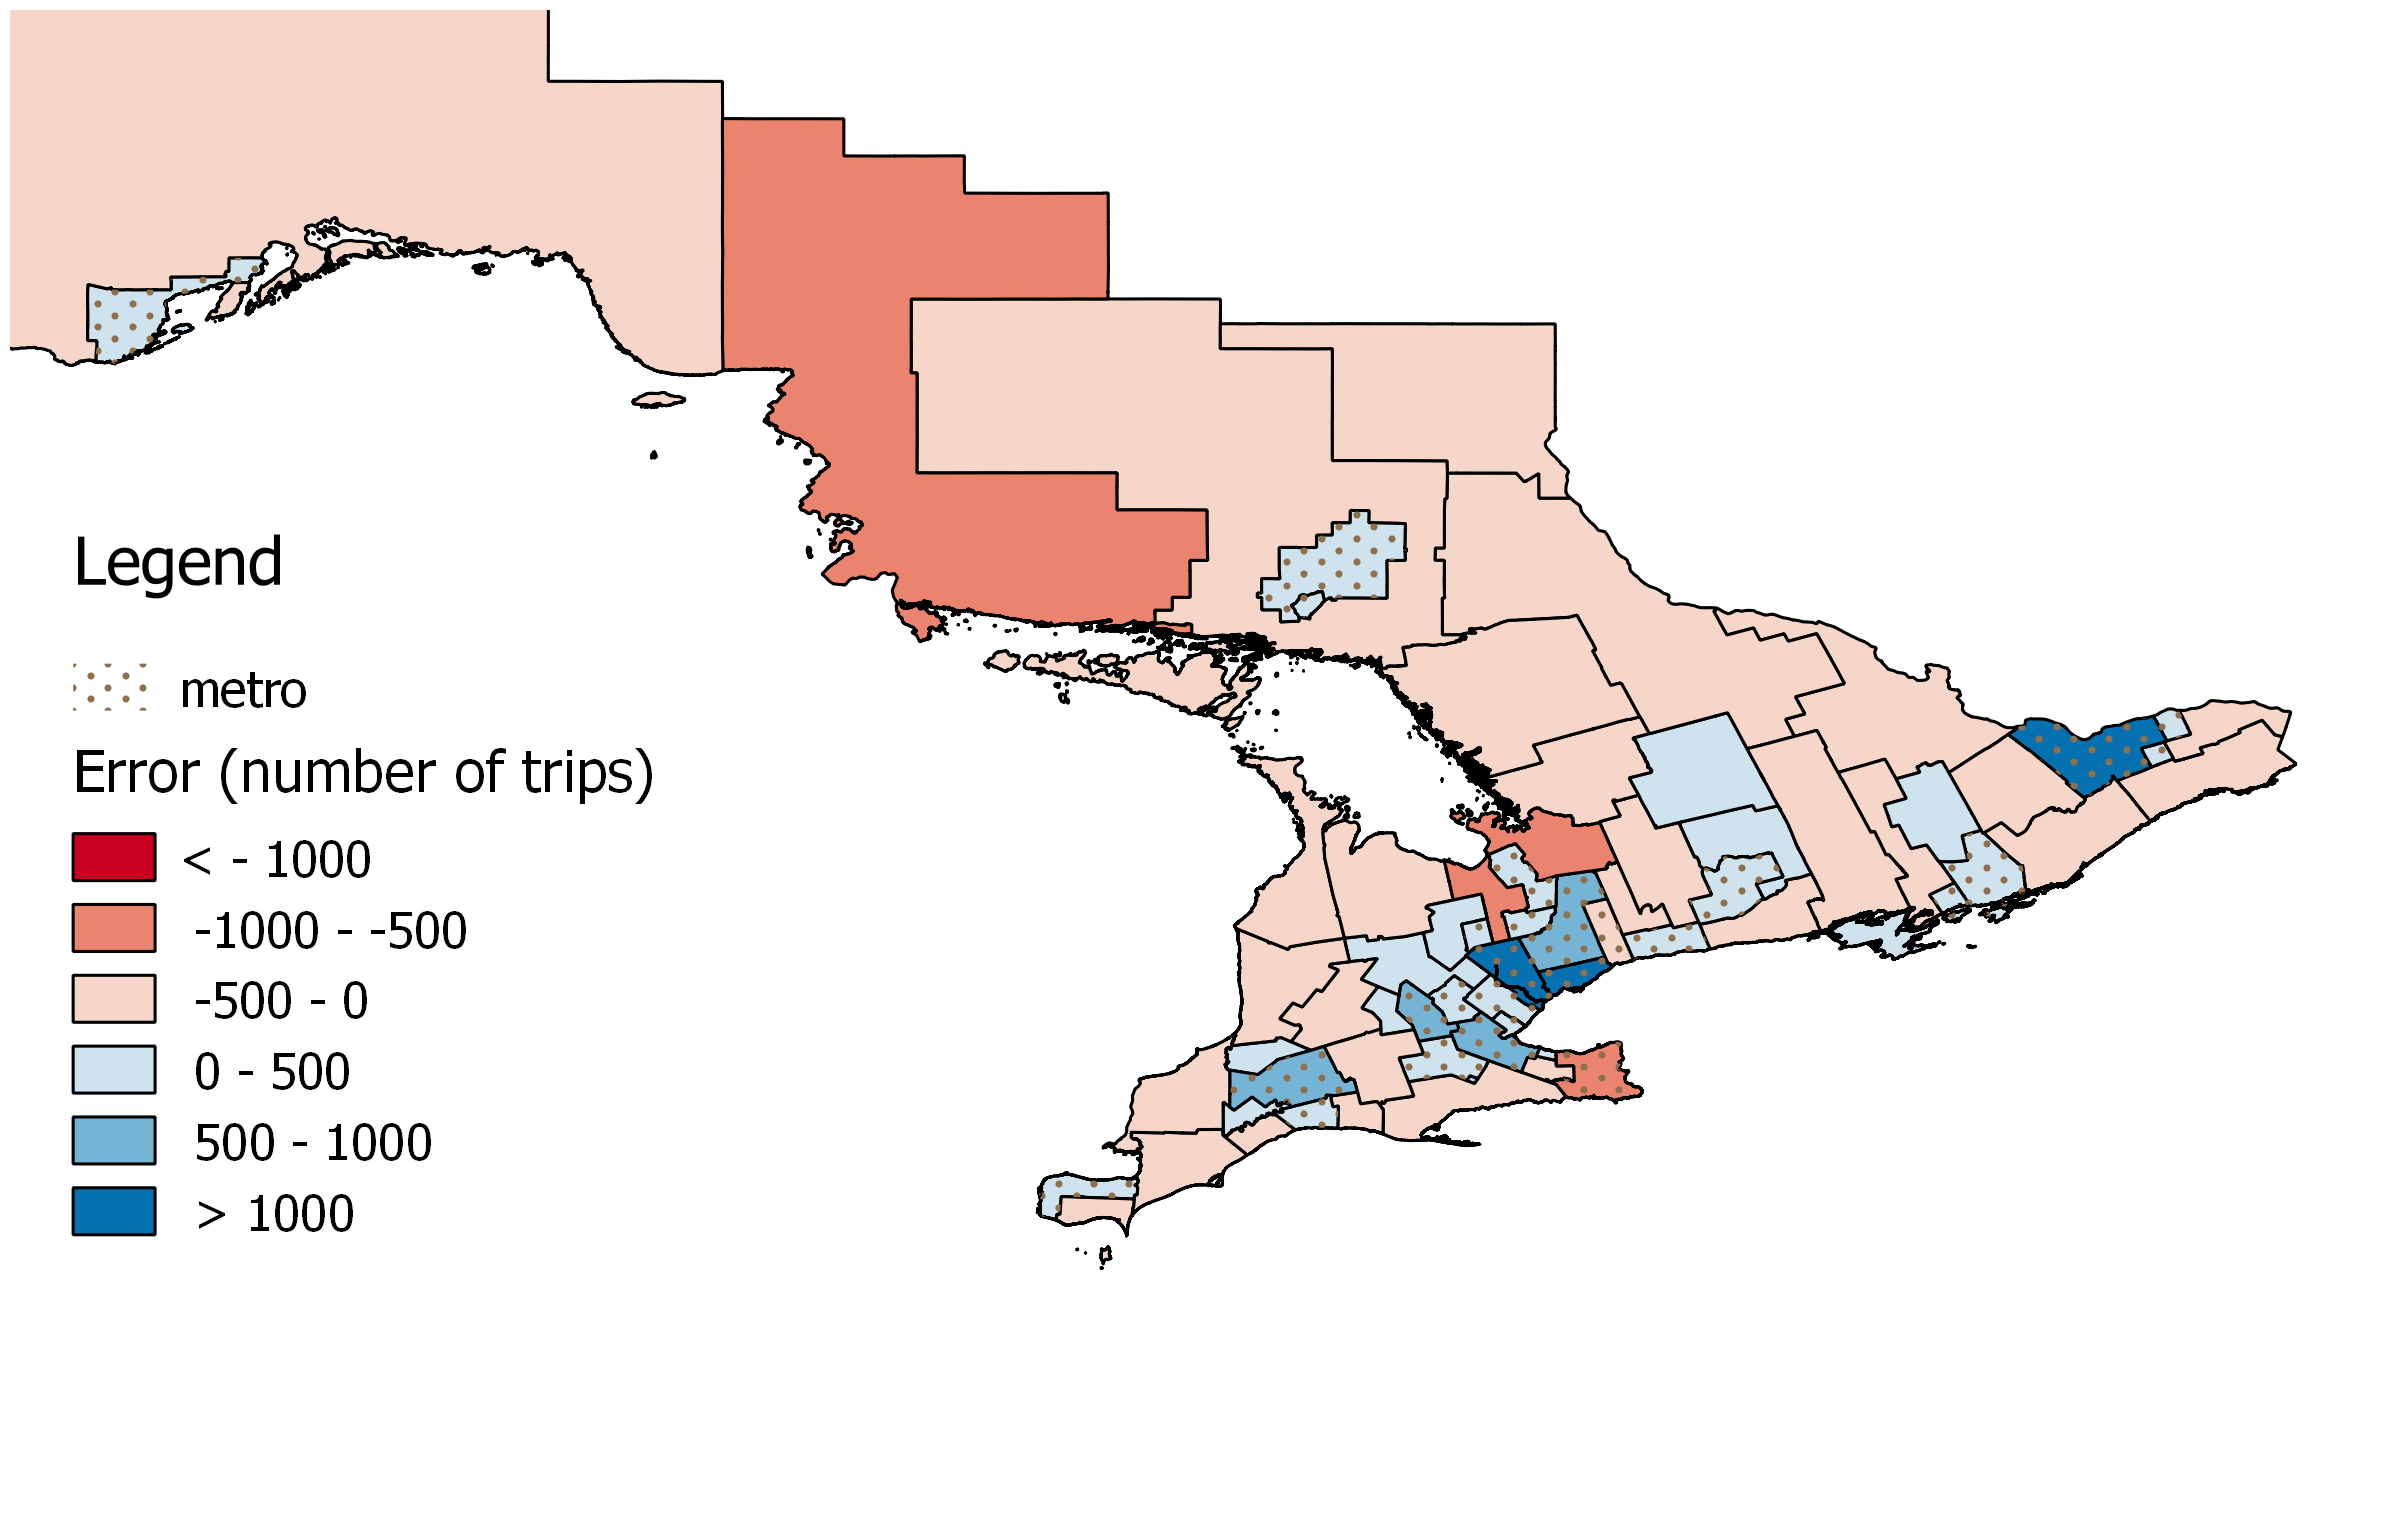
\includegraphics[width=\textwidth]{intrazonal_errors}
\caption{Intrazonal errors produced by the \textit{m2} model}
\label{fig:m2-intrazonal}
\end{figure}

\chapter{Further model results}

\begin{figure}[H]
\centering
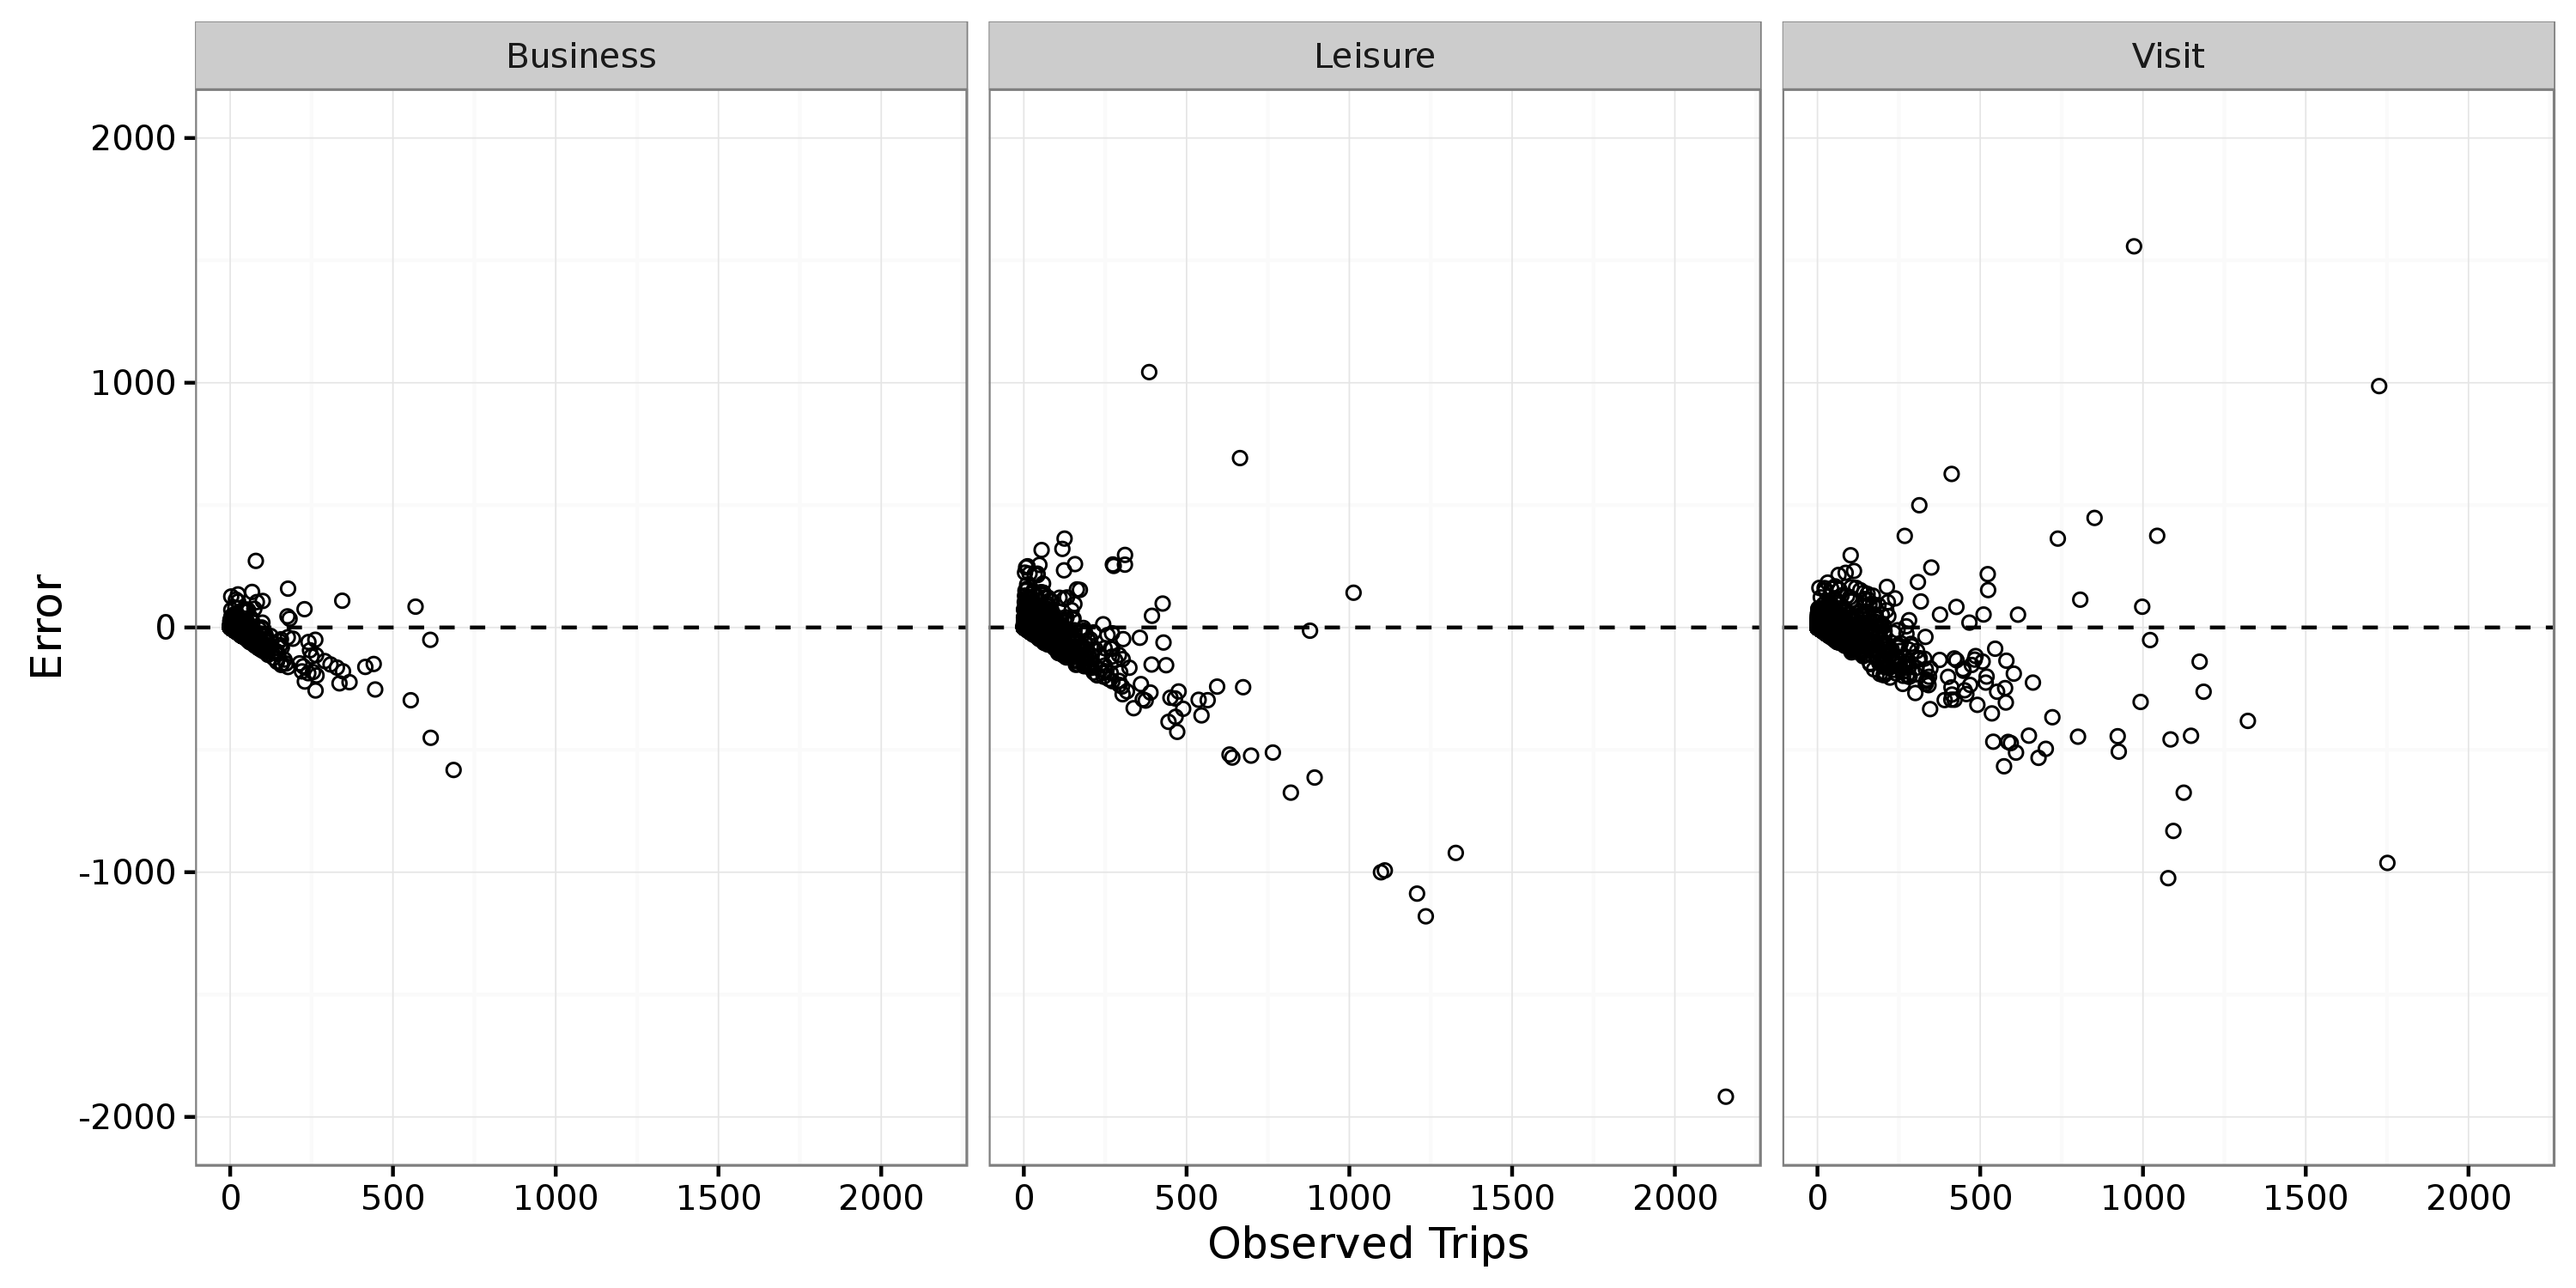
\includegraphics[width=\textwidth]{m3_residuals}
\caption{\textit{m3} model errors by observed trip count for OD pairs by trip purpose}
\label{fig:m3_residuals}
\end{figure}



	% Appendix Title

%\input{Appendices/AppendixB} % Appendix Title

%\input{Appendices/AppendixC} % Appendix Title

\addtocontents{toc}{\vspace{2em}}  % Add a gap in the Contents, for aesthetics
\backmatter

%% ----------------------------------------------------------------
\label{Bibliography}
\lhead{\emph{Bibliography}}  % Change the left side page header to "Bibliography"
\printbibliography
\end{document}  % The End
%% ----------------------------------------------------------------